\documentclass[10pt]{article}
\usepackage{icmlko}

\icmlmeta{IP 파운데이션 월드모델}{3}{294건이 86개 값으로}{주최자 발표는 측정인가 어휘인가}

\begin{document}

\twocolumn[
\icmlheader

\begin{abstract}
연구 노트 1과 2는 라벨 풀이 서로 다른 물리량을 담고 있으며, 주최자 발표 수치가 현장
게이트 계수보다 2.75배 높다는 것을 보였다. 이 노트는 그 발표 수치를 학습 타깃으로 쓸 수
있는지 묻는다. 답은 아니오이며, 이유는 편향이 아니라 \textbf{이산화}다. 주최자 발표
294건의 서로 다른 값은 86개뿐이고, 상위 12개 값이 전체의 57\%를 차지한다 --- 1만 명이
29회, 2만 명이 24회, 1만 5천 명이 20회 반복된다. 같은 라벨의 유효숫자는 95\%가 두 자리
이하다. 반면 게이트 계수 49건은 \emph{반복된 값이 하나도 없고} 유효숫자 중앙값이 네
자리다. 주최자 발표는 연속적인 측정이 아니라 몇십 개의 표현 중에서 고른
\textbf{서사적 어휘}다. 이 이산성은 역설적인 효과를 낳는다 --- 발표 수치만 모은 풀은
상수 예측 오차가 0.2656으로 가장 낮아 \emph{가장 쉬운 문제}처럼 보이지만, 그것은 예측이
쉬워서가 아니라 타깃이 몇 개 점에 몰려 있어서다. 실제 계수만 모은 풀의 상수 오차는
0.4427로 1.7배 높다. 우리가 지금까지 측정해 온 ``모델 성능''의 일부는 발표 관행을
학습한 결과였다.
\end{abstract}
]

\section{남은 물음}

앞선 두 노트에서 확인한 것을 요약한다. 라벨 풀은 우리가 직접 운영한 팝업의 현장 계수와
언론에 보도된 주최자 발표를 섞어 담고 있다. 두 집단의 중앙값은 2.75배 벌어져 있고, 같은
행사를 두 방식으로 잰 사례에서는 6.9배까지 갈렸다(노트 1). 발표 수치끼리는 서로 잘
맞으므로 그 격차는 잡음이 아니라 체계적 편향이다(노트 2).

여기서 실용적인 물음이 남는다. \textbf{발표 수치는 편향돼 있을 뿐 여전히 신호를
담고 있는가?} 만약 발표 값이 실제 수요에 비례해 부풀려진 것이라면, 로그 축에서 상수를
더한 것과 같으므로 상대적 순서는 보존된다. 그렇다면 우리는 발표 수치를 그대로 학습에
쓰되 도메인 표시자만 넣으면 된다.

이 노트는 그 가정을 검증한다.

\section{같은 숫자가 반복된다}

294건의 주최자 발표에서 서로 다른 값이 몇 개인지 세었다. 답은 86개다.

\begin{table}[t]\centering\tsize
\caption{주최자 발표에서 가장 자주 나오는 값. 상위 12개가 294건의 57\%를 차지한다.}
\label{tab:top}
\begin{tabular}{rrr}
\toprule
값 & 횟수 & 누적 \\
\midrule
10{,}000명 & 29 & 10\% \\
20{,}000명 & 24 & 18\% \\
15{,}000명 & 20 & 25\% \\
3{,}000명 & 15 & 30\% \\
5{,}000명 & 15 & 35\% \\
30{,}000명 & 12 & 39\% \\
12{,}000명 & 11 & 43\% \\
100{,}000명 & 10 & 46\% \\
50{,}000명 & 9 & 49\% \\
1{,}000명 & 8 & 52\% \\
8{,}000명 & 8 & 55\% \\
40{,}000명 & 8 & 57\% \\
\bottomrule
\end{tabular}
\end{table}

같은 물음을 게이트 계수 49건에 던지면 답이 다르다. \textbf{두 번 이상 나온 값이 하나도
없다.} 49건이 전부 서로 다른 숫자다 --- 2{,}305명, 9{,}567명, 6{,}705명처럼.

\begin{figure*}[t]\centering
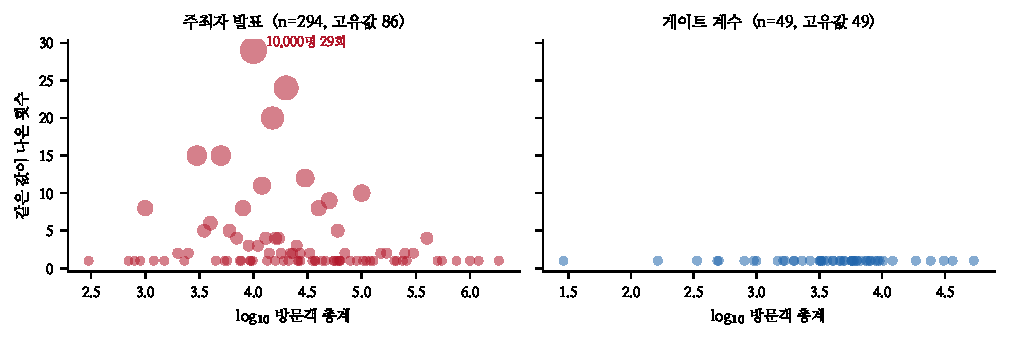
\includegraphics[width=\linewidth]{figs/value_lexicon.pdf}
\caption{값의 반복. 가로축은 방문객 총계(로그), 세로축은 그 값이 나온 횟수이며 점 크기도
횟수에 비례한다. 왼쪽 주최자 발표는 몇 개 값에 수직으로 쌓이고, 오른쪽 게이트 계수는
전부 바닥에 한 겹으로 깔린다.}
\label{fig:lex}
\end{figure*}

\claimx{주최자 발표는 연속 측정이 아니라 이산 어휘다. 294건의 고유값이 86개(29\%)이고
상위 12개가 57\%를 차지한다. 게이트 계수 49건은 고유값이 49개(100\%)다.}
{발표 수치가 몰리는 것이 어휘 때문이 아니라 실제 수요 분포가 그렇기 때문일 수 있다.
그러나 그렇다면 게이트 계수도 같은 값에 몰려야 한다. 두 집단이 같은 종류의 팝업을
대상으로 하는지는 별도 확인이 필요하다.}

\section{유효숫자가 정보량을 말한다}

값의 반복은 반올림의 결과다. 이를 직접 재기 위해 각 라벨의 유효숫자 자릿수를 세었다
--- 20{,}000은 한 자리, 15{,}000은 두 자리, 2{,}305는 네 자리다.

\begin{figure}[t]\centering
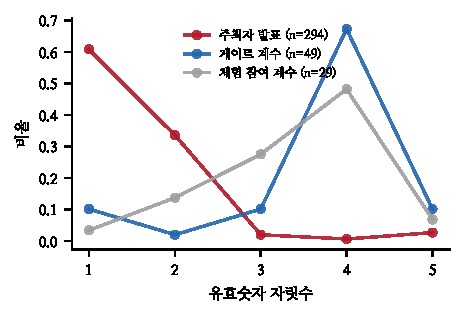
\includegraphics[width=\linewidth]{figs/sig_digits.pdf}
\caption{유효숫자 분포. 주최자 발표는 한 자리에 몰리고, 두 계수 계열은 네 자리에 몰린다.}
\label{fig:sig}
\end{figure}

\begin{table}[t]\centering\tsize
\caption{집계 기준별 유효숫자와 값의 다양성.}
\label{tab:sig}
\begin{tabular}{lrrrr}
\toprule
집계 기준 & $n$ & 1자리 & $\le$2자리 & 고유값 \\
\midrule
주최자 발표 & 294 & 61\% & 95\% & 29\% \\
게이트 계수 & 49 & 10\% & 12\% & 100\% \\
체험 참여 계수 & 29 & 3\% & 17\% & 100\% \\
\bottomrule
\end{tabular}
\end{table}

\claimx{주최자 발표의 95\%가 유효숫자 두 자리 이하다. 게이트 계수는 유효숫자 중앙값이
네 자리이며 두 자리 이하는 12\%뿐이다.}
{유효숫자는 보도 관행의 산물일 수도 있다. 주최사가 정밀한 숫자를 알면서도 기사에는
반올림해 전달할 수 있다. 그렇다면 원 수치를 얻을 경로가 있는지가 다음 물음이 된다.}

유효숫자 두 자리는 로그 축에서 무엇을 뜻하는가. 1만 명과 2만 명 사이에는 아무 값도
없으므로, 그 구간의 해상도는 $\log_{10}(2) = 0.301$이다. 우리 모델의 현재 오차가
$0.375$인 것을 생각하면, \textbf{라벨의 눈금 간격이 모델 오차와 같은 자릿수}다.

\section{이산성이 만드는 착시}

이 이산화는 실용적으로 심각한 결과를 낳는다. 라벨 풀을 집계 기준별로 나누어 상수
중앙값 예측의 오차를 재면 다음과 같다.

\begin{figure}[t]\centering
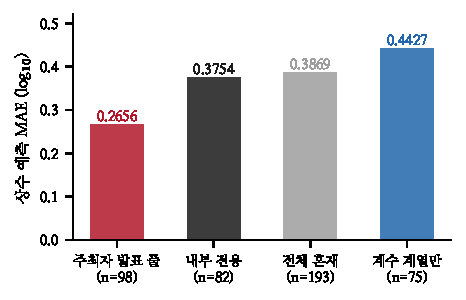
\includegraphics[width=\linewidth]{figs/pool_difficulty.pdf}
\caption{풀별 상수 예측 오차. 주최자 발표 풀이 가장 낮다. 그러나 그것은 예측이 쉬워서가
아니라 타깃이 몇 개 값에 몰려 있어서다.}
\label{fig:diff}
\end{figure}

주최자 발표만 모은 풀의 상수 오차는 $0.2656$으로 네 풀 중 가장 낮다. 표면적으로는
``가장 예측하기 쉬운 문제''로 보인다. 그러나 그 낮은 오차의 출처는 신호가 아니라
\textbf{타깃의 이산성}이다. 값이 1만·2만·3만에 몰려 있으면 중앙값 하나로도 상당수를
맞힐 수 있다.

반대로 실제 계수만 모은 풀(게이트 계수 + 체험 참여 계수, $n{=}75$)의 상수 오차는
$0.4427$로 1.7배 높다. 이것이 우리가 실제로 풀어야 하는 문제의 난이도다.

\claimx{발표 수치 풀의 낮은 오차(0.2656)는 문제가 쉬워서가 아니라 타깃이 이산적이기
때문이다. 실제 계수 풀의 상수 오차는 0.4427로 1.7배 높다.}
{두 풀은 표본 크기와 팝업 유형이 다르다. 발표 풀 98건은 언론에 보도될 만큼 규모가 큰
팝업에 치우쳐 있고, 계수 풀 75건은 우리가 운영한 것에 한정된다. 난이도 차이 중 얼마가
이산성이고 얼마가 표본 구성인지는 분리하지 못했다.}

\section{그래서 발표 수치를 쓸 수 있는가}

노트 서두의 물음으로 돌아간다. 발표 수치가 실제 수요에 비례해 부풀려진 것이라면
로그 축의 상수 이동이므로 순서는 보존되고, 도메인 표시자를 넣으면 학습에 쓸 수 있다.

그러나 이산화는 비례 관계가 아니다. 실제 수요가 1만 1천 명이든 1만 8천 명이든 발표는
``약 2만 명''으로 같아진다. 이는 상수 이동이 아니라 \textbf{정보의 소실}이다.
소실된 정보는 어떤 모델로도 복원되지 않는다.

더 나쁜 것은, 이산화가 균일하지 않다는 점이다. 작은 팝업은 ``3천 명''처럼 비교적 촘촘한
격자에 놓이지만 큰 팝업은 ``10만 명''처럼 성긴 격자에 놓인다. 즉 \textbf{라벨의 해상도가
값의 크기에 따라 달라진다}. 이런 타깃으로 학습하면 모델은 규모에 따라 다른 정밀도를
배우게 되고, 그 차이는 수요의 성질이 아니라 보도 관행에서 온다.

\claimx{발표 수치는 편향된 측정이 아니라 정보가 소실된 측정이다. 비례 보정으로
복원할 수 없으며, 해상도가 값의 크기에 따라 달라져 규모별 정밀도까지 왜곡한다.}
{소실 여부는 원 수치와 대조해야 확정된다. 주최사가 정밀 수치를 보유하는지, 그것을
얻을 경로가 있는지 확인하지 못했다. 만약 다수 사례에서 원 수치를 얻을 수 있다면
이 결론은 ``현재 수집 경로의 한계''로 축소된다.}

\section{그러면 무엇이 남는가}

학습 타깃으로 쓸 수 있는 것은 계수 계열 75건이다. 이는 우리가 다뤄 온 427건의 18\%다.

이 결론은 불편하지만 앞선 두 노트와 일관된다. 노트 1은 혼재 풀에서의 성능 측정이
해석 불가능함을 보였고, 노트 2는 그 혼재가 스코프와 시점에서도 일어남을 보였다.
노트 3은 발표 수치가 편향을 넘어 정보 자체를 잃었음을 보인다.

세 노트가 공통으로 가리키는 것은 하나다. \textbf{이 프로젝트의 병목은 모델도 피처도
아니고 라벨이다.} 그리고 라벨을 늘리는 방향이 아니라 \emph{정의를 세우는} 방향이어야 한다.

\section{다음 단계}

\paragraph{즉시}
계수 계열 75건만으로 학습 파이프라인을 재구성하고, 그 위에서 피처 절제를 다시 검정한다.
현재 132개 피처는 이 표본 크기에 명백히 과하다.

\paragraph{라벨 확보}
발표 수치를 계수로 바꿀 경로를 찾는다. 우리가 운영한 팝업은 이미 계수가 있고, 운영하지
않은 팝업은 웨이팅 시스템 로그나 유통사 층별 집계 같은 원 데이터가 있어야 한다.
이는 기술이 아니라 접근 권한의 문제다.

\paragraph{측정 규율}
발표 수치를 완전히 버릴 필요는 없다. 다만 \emph{다른 타깃}으로 다뤄야 한다 --- ``이 팝업이
얼마나 화제가 될 것인가''는 ``몇 명이 올 것인가''와 다른 질문이고, 발표 수치는 전자에
더 가깝다. 두 질문을 분리하면 발표 수치 294건도 쓸 자리가 생긴다.

\vspace{0.7em}
\hrule
\vspace{0.4em}
{\footnotesize\color{black!60}
모든 수치는 저장소 데이터에서 그림 생성 코드가 직접 계산한다.
재현: \texttt{python3 paper/figs.py}. 라벨이 갱신되면 그림과 표도 함께 바뀐다.}

\end{document}
